% !TeX spellcheck = en_US

\chapter{Implementação da Base de Dados}

Um protótipo de uma Base de Dados de WhiteSpace (BDWS)
\abbrev{BDWS}{Bases de Dados de WhiteSpace}
foi implementado anteriormente por Marcelo Machado em seu trabalho de conclusão de curso~\cite{tccmarcelo}. Essa base é capaz de indicar a um US os canais livres no espectro de frequência, permitindo sua utilização. Para isso, a base possui informações sobre todos os UPs presentes. É passado como parâmetro de entrada a localização do US e a base retorna uma resposta com a lista de canais disponíveis para uso.

O espectro de frequência é extenso e utilizado para várias finalidades, como Transmissão de dados para satélites, rádio navegação e transmissão de TV. Atualmente, a base implementada possui apenas informações referentes ao espectro de transmissão de TV, que vai de 54 Mhz até 806Mhz~\cite{fccalloc} .

A base possui as informações referentes às antenas de televisão que operam na região do Estado do Rio de Janeiro. Esses dados foram obtidos da ANATEL~\cite{channelstable}. Certos dados oriundos da agência reguladora estão incompletos e inconsistentes, o que acarreta erros de cálculo na base. Torna-se necessária uma maior cooperação entre a agência reguladora com a base, para aumentar a confiabilidade das respostas às requisições dos USs.

\section{Tecnologias Utilizadas}

O sistema foi desenvolvido utilizando a linguagem de programação orientada a objetos Java, com o Sistema de Gerenciamento de Banco de Dados MYSQL
\abbrev{SGBD}{Sistema de Gerenciamento de Banco de Dados} 
para armazenamento dos dados. O protocolo utilizado para o desenvolvimento da  Application Programming Interface (API)
\abbrev{API}{Application Programming Interface} 
foi o REST, para isso, foi utilizada uma biblioteca Java chamada Restlet~\cite{restlet}. As respostas do sistema são no formato XML ou no formato JSON. O desenvolvimento da base foi realizado no ambiente Eclipse.

A aplicação Web utilizou  HyperText Markup Language(HTML)
\abbrev{HTML}{HyperText Markup Language}
para produção das páginas Web, em conjunto com a linguagem script Javascript para dinamização. Para customizar o layout da página, foi utilizado Cascading Style Sheets(CSS)
\abbrev{CSS}{Cascading Style Sheets}
como linguagem de estilo. Para realização de requisições assíncronas ao servidor, utilizou-se o AJAX. Por fim, para renderização do mapa geográfico na página Web, foi utilizada a API em Javascript de mapas HERE~\cite{heremaps}. 

\section{Arquitetura do Servidor}

Como citado na seção anterior, o servidor realiza a consulta ao banco de dados e obtém as informações dos UPs, em seguida aplica um dos modelos de propagação implementados e retorna uma lista com os canais livres baseada na posição geográfica do US.

\subsection{Cálculo dos Canais Disponíveis}

O servidor consulta o banco de dados e coleta as informações das antenas presentes no Estado do Rio de Janeiro. A partir de sua altura e potência, calcula-se o alcance máximo para cada antena, dependendo do modelo de propagação do sinal. O alcance máximo é definido como: "A distância máxima da base da antena que um dispositivo pode estar para receber o sinal transmitido por ela com uma relação sinal/ruído mínima. Assume-se que o dispositivo não sofre nenhuma interferência além de duas vezes ruído de fundo". Os dispositivos que possuírem uma distância menor que o raio da antena, receberão o sinal com qualidade suficiente. Já os dispositivos com distancia da antena maior que seu raio, estarão fora do alcance da mesma, podendo utilizar esse canal para transmissão de seus dados. Essa condição é necessária para que um US possa transmitir dados nessa frequência sem causar interferências.

Assumindo um Usuário Primário P com alcance \begin{math}p\end{math} e um Usuário Secundário S com alcance \begin{math}s\end{math}. Sendo D a distância entre P e S. O US S poderá transmitir dados utilizando o canal de P somente se:

\begin{align}
  \label{cantransmitdata} p + s > D
\end{align}

Os alcances \begin{math} p \end{math} e \begin{math} s \end{math} são obtidos através dos modelos de propagação implementados na base. Os modelos que foram implementados anteriormente são: 

\begin{itemize}
\item Free Space
\item Two Ray Ground
\item Log Distance
\end{itemize}

\subsubsection{Modelos de Propagação Implementados}

Cada modelo retorna um valor de atenuação, no qual a relação sinal/ruído se torna igual a 10dB. Esse modelo é aplicado tanto para o UP quanto para o US, e com isso, encontra-se a distância máxima do alcance de um dispositivo. Para isso, é necessário encontrar a relação sinal/ruído, definida:

\begin{align}
  \label{Sinr} SINR=\frac{P}{I+N}
\end{align}

Onde \textit{P} é a potência do sinal, \textit{I} é a interferência e \textit{N} é o ruído de fundo.

Como é assumido que a única interferência no ambiente será o ruído de fundo, tem-se então que:

\begin{align}
  \label{actSinr} SINR=\frac{P}{N}
\end{align}

O ruído de fundo, em Watts, é definido como:

\begin{align}
  \label{noise} Noise=kTB
\end{align}

Aonde \textit{k} é a constante de Boltzman, \textit{T} é a temperatura do ambiente e \textit{B} é a banda em hertz.

Assim, pelas equações~\ref{actSinr} e~\ref{noise} tem-se que a potência mínima do receptor é:

\begin{align}
  \label{minPot} P_r= SINR \cdot  kTB
\end{align}

O valor da relação sinal/ruído deve ser convertido para W de forma a facilitar os cálculos. Dessa forma:

\begin{align}
  \label{SinrW} 10= 10 log_{10} (SINR_W)
\end{align}

De modo que a potência do sinal emitido pela antena em seu alcance máximo será:

\begin{align}
  \label{minPotAnt} P_{a}= 10kTB
\end{align}

 No entanto, o dispositivo que utiliza o WS não pode interferir com os receptores da antena. Dessa forma, seu sinal deve ser atenuado até atingir o valor do ruído de fundo. Assim sendo, a relação sinal/ruído deve ser de 0dB. De modo que podemos determinar a potência no alcance máximo do dispositivo como sendo:

\begin{align}
  \label{minPotDev} P_{d}=  kTB
\end{align}

\subsubsection{Free Space}

O modelo de propagação Free Space assume que o transmissor e o receptor possuem um caminho em linha reta, sem obstáculos próximos que possam causar os fenômenos de difração ou interferência. Esse modelo raramente é utilizado exclusivamente, normalmente faz parte de um modelo maior, como o Longley-Rice. Por desconsiderar as irregularidades do solo e assumir que o meio é sem obstrução, os alcances acabam sendo muito maiores do que a realidade. O modelo é ilustrado na figura abaixo\ref{fig:freespaces}.

\begin{figure}[htb]
\centering
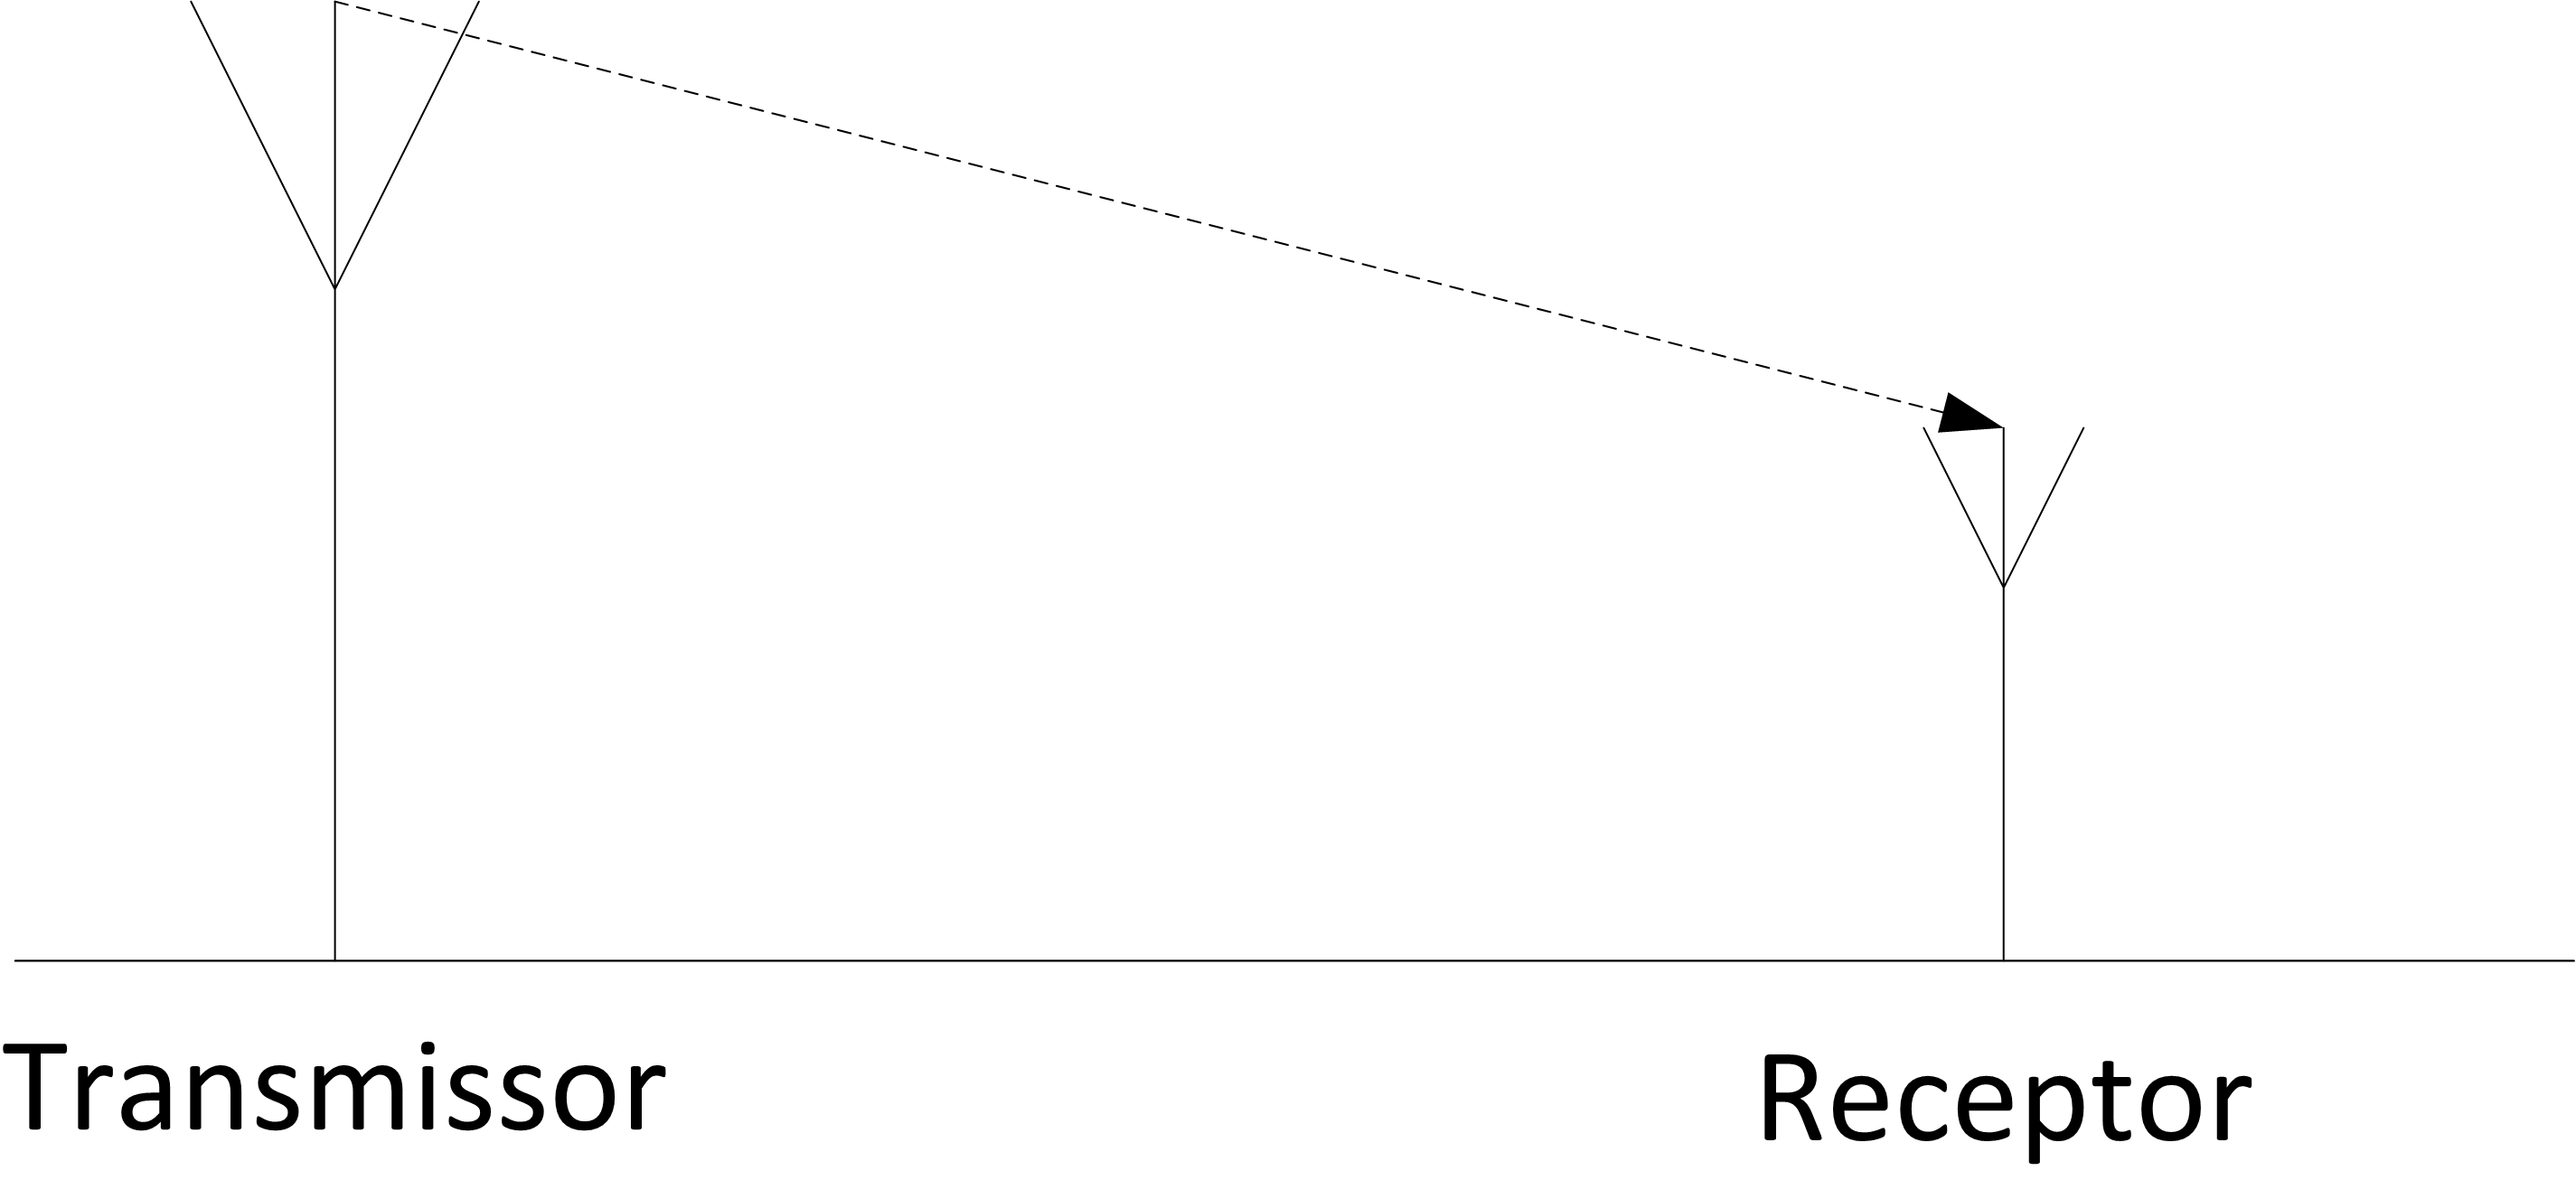
\includegraphics[width=0.8\textwidth]{figs/freespaces}
\caption[Modelo de propagação Free Space.]
{Modelo de propagação Free Space.}
\label{fig:freespaces}
\end{figure}

A potência recebida pelo receptor quando o transmissor se encontra a uma distância \textit{d} é definida~\cite{rapapport} como: 

\begin{align}
  \label{potfree} P_r(d) =\frac{ P_tG_tG_r\lambda^{2}}{(4\pi)^{2}d^{2}L}
\end{align}

\begin{math}G_t\end{math} e \begin{math}G_r\end{math} são os ganhos do transmissor e receptor respectivamente. Foi assumido que a potência indicada pela ANATEL é, na verdade, \begin{math}P_tG_t\end{math}, enquanto \begin{math}G_r\end{math} foi desconsiderado.

\begin{align}
  \label{ganho} G_r = 1
\end{align}

\textit{L} representa o fator de perda não relacionado ao modelo de propagação. L também foi desconsiderado.

\begin{align}
  \label{loss} L = 1
\end{align}

\begin{math}\lambda\end{math} é referente a frequência utilizada para transmissão, onde \textit{c} é a velocidade da luz em m/s e \textit{f} é a frequência utilizada em Hz.

\begin{align}
  \label{lambda}\lambda=\frac{c}{f}
\end{align}

Assim sendo, determina-se o alcance de uma antena no modelo de Free Space pelas equações~\ref{potfree} e~\ref{minPotAnt}:

\begin{align}
  \label{dFreeAnt} d_1 = \sqrt{\frac{P_t\lambda^{2}}{10kTBL(4\pi)^{2}}}
\end{align}

De maneira análoga, o alcance de um US pode ser determinado pelas equações~\ref{potfree} e~\ref{minPotDev}:

\begin{align}
  \label{dFreeDev} d_2 = \sqrt{\frac{P_t\lambda^{2}}{kTBL(4\pi)^{2}}}
\end{align}

\subsubsection{Two Ray Ground}

\begin{figure}[htb]
\centering
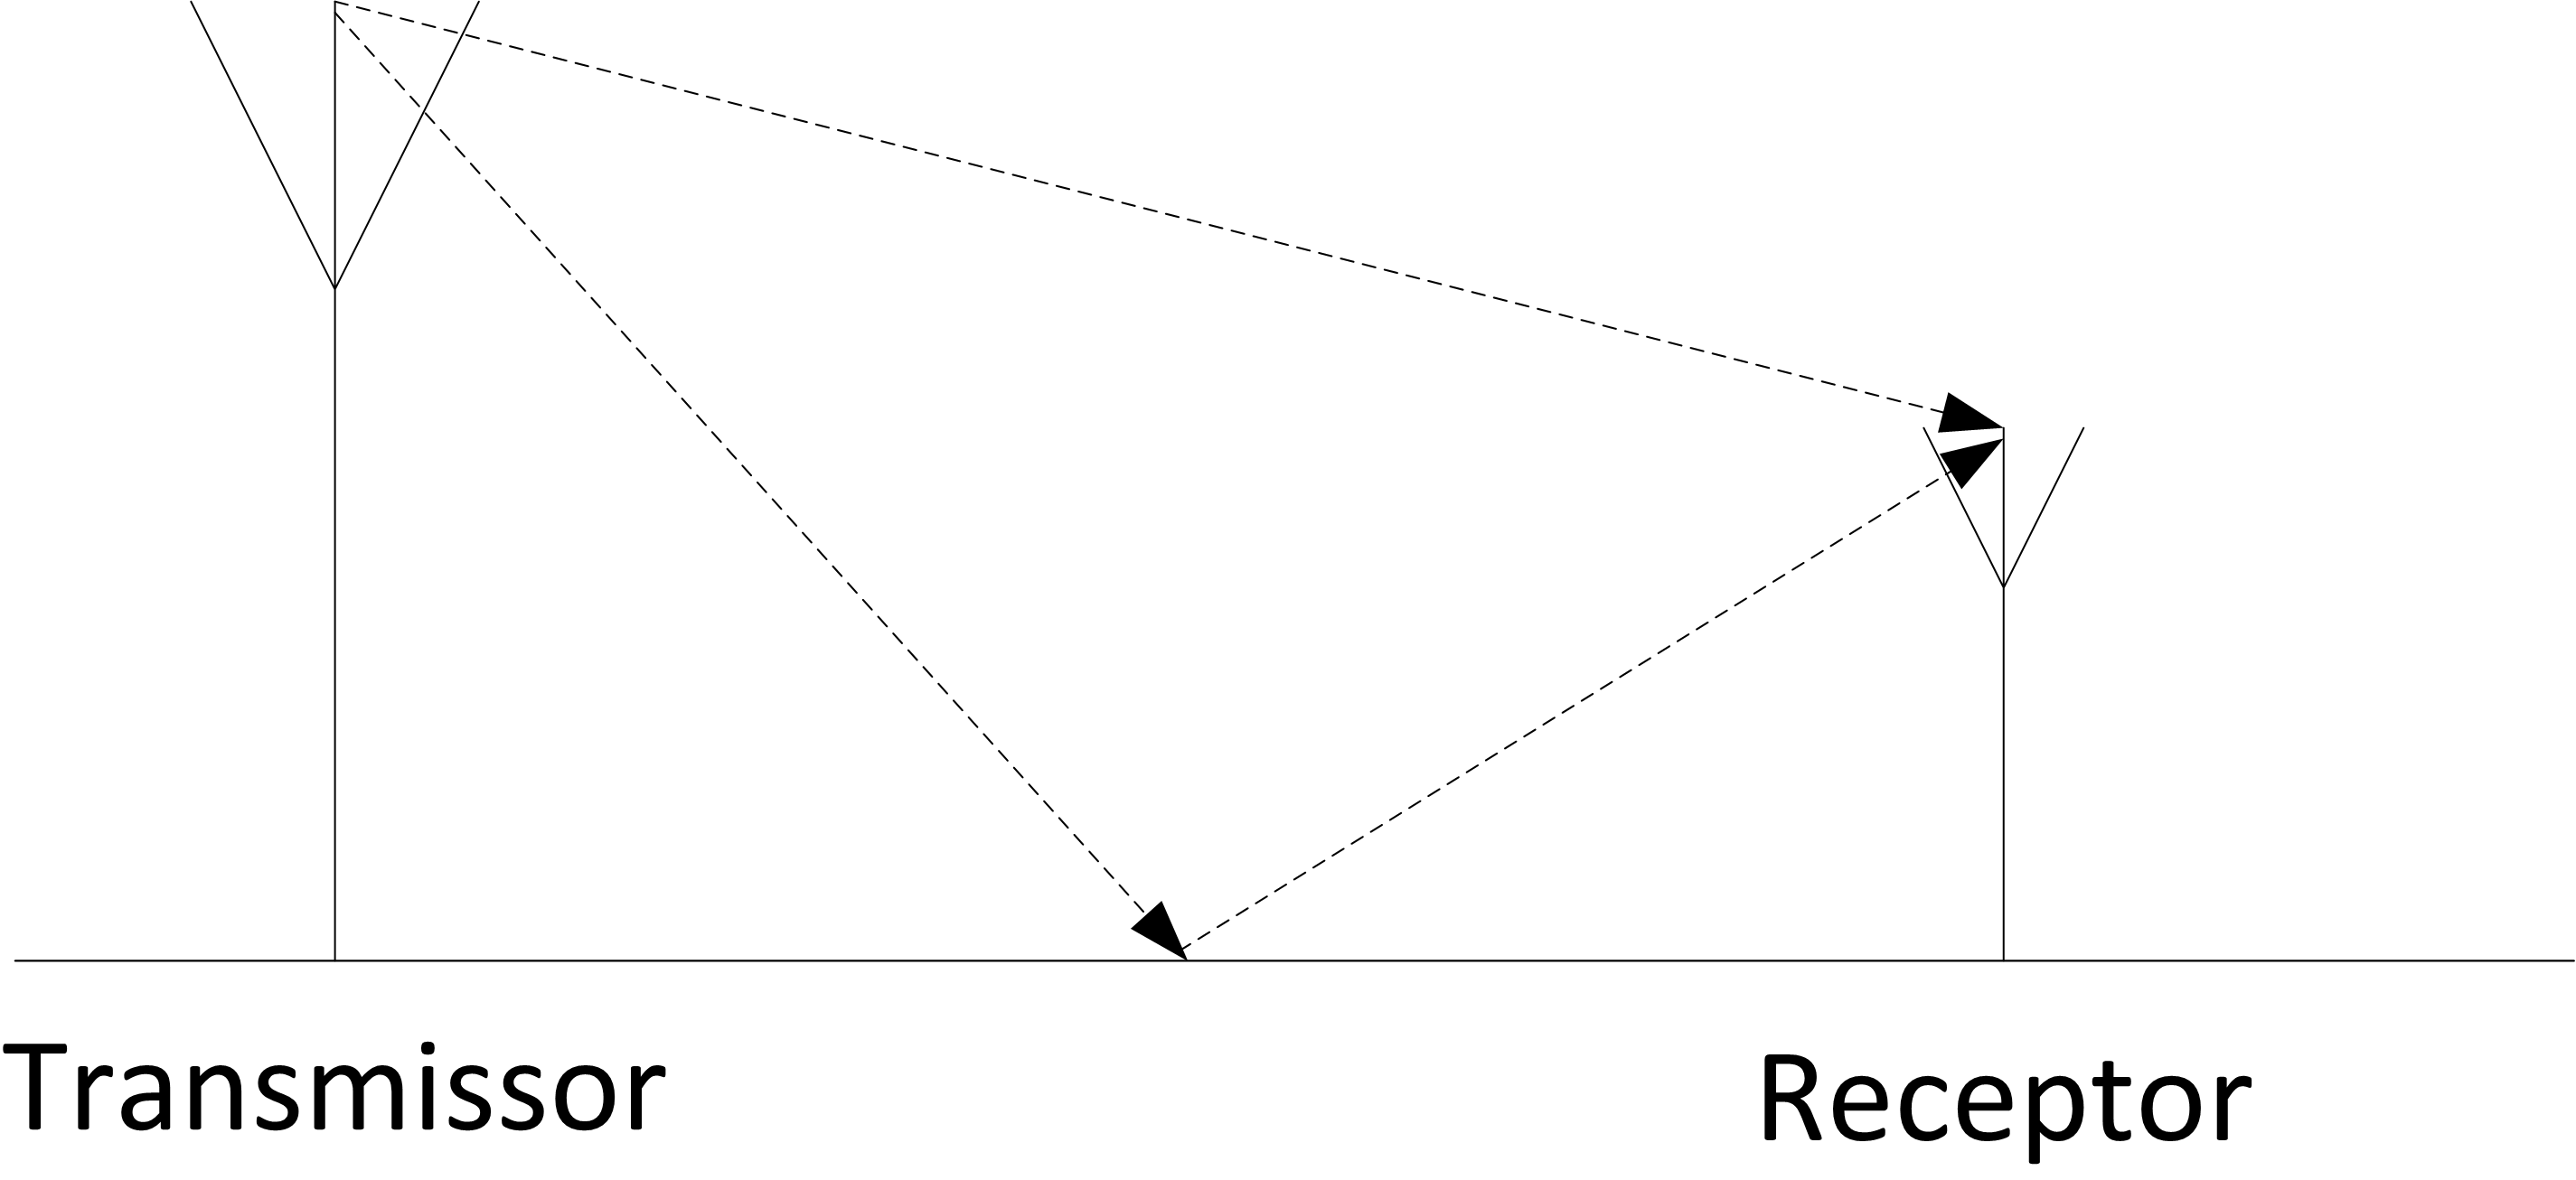
\includegraphics[width=0.8\textwidth]{figs/tworay}
\caption[Modelo de propagação Two Ray Ground.]
{Modelo de propagação Two Ray Ground.}
\label{fig:tworay}
\end{figure}

O modelo Two Ray Ground leva em consideração dois caminhos: O primeiro é equivalente ao Free Spaces, ou seja, um caminho direto do transmissor ao receptor e o segundo é um caminho que incide no solo e é refletido para o receptor. Um exemplo é ilustrado na figura~\ref{fig:tworay}.

A potência recebida pelo receptor quando o transmissor se encontra a uma distância \textit{d} é definida~\cite{rapapport} como: 

\begin{align}
  \label{pottworay} P_r(d) = P_tG_tG_r\frac{h_t^{2}h_r^{2}}{d^4}
\end{align}

Onde \begin{math}h_t\end{math} é a altura da antena transmissora e \begin{math}h_r\end{math} é a altura da antena do receptor em metros. Foi assumida uma altura de 2 metros para casos onde não foi possível determinar a altura do dispositivo.

Assim, assumindo a equação~\ref{ganho}, temos, pelas equações~\ref{pottworay} e~\ref{minPotAnt} o alcance de uma antena no modelo Two Ray Ground:

\begin{align}
  \label{dTwoRayAnt} d_1 = \sqrt[4]{\frac{P_th_t^{2}h_r^{2}}{10kTB}}
\end{align}

De maneira análoga, o alcance de um US pode ser determinado pelas equações~\ref{potfree} e~\ref{minPotDev}:

\begin{align}
  \label{dTwoRayDev} d_2 = \sqrt[4]{\frac{P_th_t^{2}h_r^{2}}{kTB}}
\end{align}


\subsubsection{Log Distance}

O modelo de propagação Log Distance é bastante utilizado para longas distâncias e assume que a potência transmitida por uma antena decai logaritmicamente em relação à distância. Dois fatores principais entram em cena, a perda ocorrida a uma distância muito pequena, e a taxa de decaimento.

\begin{math}L_0\end{math} determina a perda ocorrida a uma distância muito pequena. Foi considerado a distância \begin{math}d_0\end{math} como sendo 1 metro. Essa perda foi calculada no modelo Free Space:

\begin{align}
  \label{L0} L_0 = \left( \frac{4\pi w}{c}\right)^{2}
\end{align}

Onde \begin{math}w\end{math} é o comprimento de onda da freqência utilizada e \begin{math}c\end{math} é a velocidade da luz em metros.

O modelo foi simplificado de forma que o alcance de uma antena é representado por:

\begin{align}
  \label{dLogDistAnt} d_1 = \sqrt[\gamma]{\frac{d_0^{\gamma}10^{\frac{-L_0}{10}}  P_t}{10kTB}}
\end{align}

De maneira análoga, o alcance de um US é representado por:
\begin{align}
  \label{dLogDistDev} d_2 = \sqrt[\gamma]{\frac{d_0^{\gamma}10^{\frac{-L_0}{10}}  P_t}{kTB}}
\end{align}

\begin{math}\gamma \end{math} representa um fator de perda que geralmente recebe valores de 2 a 6. Foi escolhido 3 como sendo valor padrão.

\subsubsection{Constantes}

As seguintes constantes foram assumidas para os cálculos descritos:

\begin{itemize}
\item d =\begin{math}1380\cdot 10^{-23}\end{math}  mW
\item T = 290 K
\item B = 6 MHz
\item c = 299792458 m/s
\end{itemize}

\section{Extensão dos modelos}

Os modelos implementados não levam em conta a perda causada pelo relevo, o que pode gerar resultados menos acurados, podendo causar interferências ou subutilização de canais no espectro. Um novo modelo de propagação foi desenvolvido nesse trabalho, levando em contra outras variáveis para determinar a atenuação do sinal de um dispositivo.

\subsection{Longley-Rice}

Também conhecido como Irregular Terrain Model (ITM)\abbrev{ITM}{Irregular Terrain Model}, este modelo foi publicado por A. G. Longley e P. L. Rice em 1968.~\cite{longleyrice} Utilizado para frequências entre 20 MHz até 20GHz, foi criado para atender às necessidades do planejamento de frequências na transmissão de televisão nos Estados Unidos.

O Longley-Rice é capaz de predizer a atenuação de dois modos diferentes: O modo área e o modo ponto-a-ponto. O modo área utiliza informações médias do perfil do terreno para realizar o cálculo da atenuação. Já o modo ponto-a-ponto utiliza informações específicas do caminho entre o transmissor e o receptor para realização o cálculo da atenuação.
Também possui estimativas da variabilidade do tempo e localização.

\subsubsection{Parâmetros de Entrada}

Para ambos os modos, os parâmetros listados abaixo são necessários:

\begin{itemize}
\item \begin{math}d\end{math} Distância entre os dispositivos
\item \begin{math}k\end{math} Número de onda
\item \begin{math}h_{g1}, h_{g2}\end{math} Altura estrutural das antenas
\item \begin{math}\Delta h\end{math} Parâmetro de irregularidade do terreno
\item \begin{math}N_s\end{math} Refratividade da Superfície
\item \begin{math}\gamma _e\end{math} Curvatura efetiva da terra
\item \begin{math}Z_g\end{math} Impedância da superfície
\item clima Expresso qualitativamente com um número para denotar um tipo de clima discreto
\end{itemize}

Para obtermos o número de onda, basta aplicarmos a fórmula:

\[
k = 2\pi/\lambda = f/f_0 \,\,\,\,\, \text{ sendo} \,\,\,\,\,\,\,\,\, f_0 = 47.70 \text{ MHz . m }
\]

O parâmetro de irregularidade do terreno pode ser obtido na tabela~\ref{table:deltah}. \\

\begin{table}[h]
\centering
\caption[Valores para o parâmetro de irregularidade do terreno.]
{Tabela obtida no relatório de Longley, Rice  e Kissick ~\cite{longleyricedelta}} 
\label{table:deltah}
\begin{tabular}{ll}

\hline
                             & $\Delta$ h (metros) \\ \hline
Plano ou sobre a água        & 0                 \\
Planícies                    & 30                \\
Colinas                      & 90                \\
Serras                       & 200               \\
Montanhas                    & 500               
\end{tabular}
\end{table}

No artigo original do modelo~\cite{longleyrice}, um programa foi apresentado e as previsões da atenuação do sinal foram testadas para um certo intervalo de valores de entrada, onde o modelo provou-se eficiente. Os parâmetros e seus respectivos intervalos estão listados na tabela~\ref{table:longleyricevaluesinterval}:\\

\begin{table}[h]
\centering
\caption[Intervalos válidos para os parâmetros de entrada.]
{Intervalos válidos para os parâmetros de entrada.}
\label{table:longleyricevaluesinterval}
\begin{tabular}{ll}
\hline
Parâmetros                  & Intervalo            \\ \hline
Frequência                  & 20 a 40,000 MHz      \\
Altura das Antenas          & 0.5 a 3,000 m        \\
Distância                   & 1 a 2,000 km         \\
Refratividade da Superfície & 250 a 400 N-unidades
\end{tabular}
\end{table}

A polarização da antena pode ser horizontal ou vertical e afeta o valor da impedância da superfície \begin{math}Z_g\end{math}, ibtida pela análise da permissividad e condutividade do solo em relação à polarização das ondas. A impedância característica do solo em relação a sua polarização é apresentada a seguir:


\[ Z_g = \begin{cases} 
      \sqrt{\epsilon_r' - 1} & \textrm{ Polarização horizontal} \\
      \frac{\sqrt{\epsilon_r' - 1}}{\epsilon_r'} & \textrm{ Polarização vertical} \\
   \end{cases} \]

onde \begin{math}\epsilon_r'\end{math} é a Permissividade relativa complexa, definida por:

\[ 
\epsilon_r' = \epsilon_r + i Z_0\sigma/k
\]
\[
Z_0 = 376.62 \textrm{ ohm.}
\]
A condutividade do solo $\sigma$ é expressa em siemens por metro. Seus possíveis valores podem são apresentados na tabela ~\ref{table:sigmainterval}

\begin{table}[h]
\caption[Valores para a permissividade relativa e condutividade do solo.]
{Valores para a permissividade relativa e condutividade do solo.}
\label{table:sigmainterval}
\centering
\resizebox{\textwidth}{!}{%
\begin{tabular}{lcc} \\
\hline
            & Permissividade Relativa & Condutividade (Siemens por metro) \\ \hline
Solo médio  & 15                      & 0.005                             \\
Solo pobre  & 4                       & 0.001                             \\
Solo bom    & 25                      & 0.020                             \\
Água fresca & 81                      & 0.010                             \\
Água do mar & 81                      & 5.0                              
\end{tabular}
}
\end{table}

A curvatura efetiva da terra $\gamma_e$ pode ser obtida através da fórmula:

\[
\gamma_e = \gamma_a/K
\]

Onde $\gamma_a$ é a curvatura real da terra e $K$ é o fator de raio efetivo da Terra. O valor normalmente é obtido através de sua formúla empírica:
\[
\gamma_e = \gamma_a(1-0.04665e^{N_s/N_1})
\]

onde

\[
N_1 = 179.3 \text{ N-unidades, e } \gamma_a = 157 . 10^-9 \text{ m} ^-1 = 157 \text{ N-unidades/km.}
\]
A refratividade da superfície \begin{math}N_s\end{math} é obtida a partir da análise das condições atmosféricas, como a temperatura, pressão e umidade relativa. Esse valor determina quantidade de sinal que é refratado pela atmosfera.
Para simplificar a sua representação, a refratividade da superfície  é definida em termos de \begin{math}N_0\end{math}, a refratividade da superfície reduzida ao nível do mar.

\[
N_s = N_0e^{-z_s/z_1} \,\,\,\,\, \text{ sendo} \,\,\,\,\,\,\,\,\, z_1 = 9.46 \text{ km }
\]
Onde \begin{math}z_s\end{math} é a elevação geral da região envolvida. Para o modo ponto-a-ponto, esse valor é a média aritmética das elevações no caminho entre o transmissor e o receptor.
Ao reduzirmos a refratividade da superfície ao nível do mar, podemos utilizar o mapa presente no relatório ~\cite{longleyricedelta} para obter um valor válido para \begin{math}N_s\end{math}. Os valores são apresentados na figura.~\ref{fig:nsmap} Esses dados podem ser resumidos em função do clima da região em estudo, listados na tabela ~\ref{table:climatetable}.



\begin{table}[h]
\centering
\caption[Refratividade da superfície em função do clima da região.]
{Refratividade da superfície em função do clima da região.}
\label{table:climatetable}
\resizebox{\textwidth}{!}{%
\begin{tabular}{lc}
\hline
Clima                       & Refratividade da superfície (N-unidades) \\ \hline
Deserto                     & 280                                    \\
Continental Temperado       & 301                                    \\
Continental Sub-tropical    & 320                                    \\
Marítimo Temperado          & 320                                    \\
Marítimo temperado sobre o mar & 350                                    \\
Equatorial                  & 360                                    \\
Marítimo Sub-tropical       & 370                                    \\
\end{tabular}
}
\end{table}

\begin{figure}[nsmap]
\centering
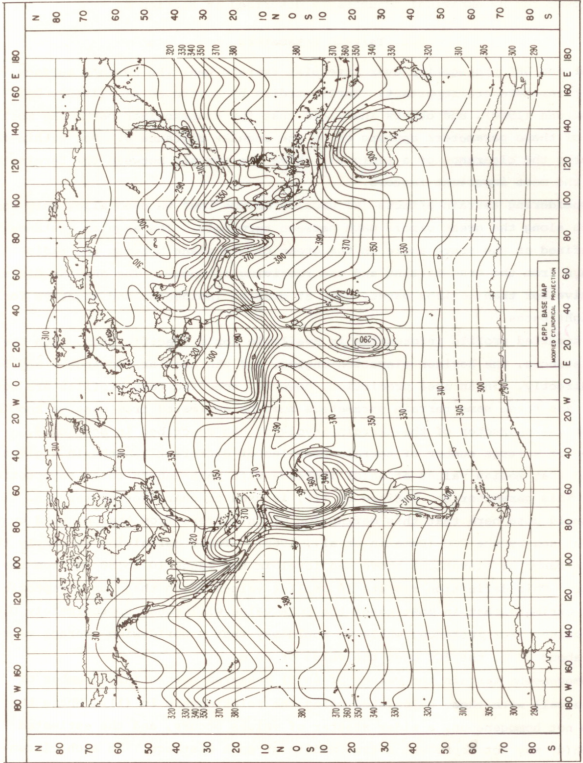
\includegraphics[width=0.8\textwidth]{figs/nsmap}
\caption[Refratividade média da superfície reduzida ao nível do mar.]
{Refratividade média da superfície reduzida ao nível do mar.}
\label{fig:nsmap}
\end{figure}

\subsubsection{Parâmetros adicionais}

Cada modo depende de diferentes parâmetros de entrada. Nesse trabalho foi implementado o modo ponto-a-ponto, no qual as informações do relevo entre o transmissor e o receptor são conhecidos.  
As variáveis adicionais utilizadas pelo algoritmo são:

\begin{itemize}
\item \begin{math}h_{eb}, h_{em}\end{math} Alturas efetivas das antenas
\item \begin{math}d_{lb},d_{lm}\end{math} Distância de cada dispositivo ao seu horizonte de radio
\item \begin{math}\theta_{eb}, \theta_{em}\end{math} Ângulos de elevação dos horizontes de cada dispositivo na altura das antenas
\end{itemize}

No modo área, esses valores são aproximados utilizando uma fórmila empírica na qual $\Deltah$ influencia fortemente.
A altura efetiva de uma antena é a altura acima de um plano refletor, os valores podem ser encontrados na figura ~\ref{fig:radiohorizon}~\cite{irregularterrain}, 

\begin{figure}[radiohorizon]
\centering
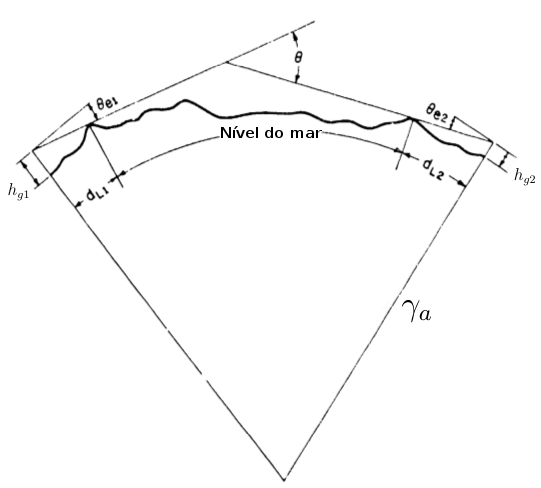
\includegraphics[width=0.8\textwidth]{figs/radiohorizon}
\caption[Variáveis do modo ponto-a-ponto.]
{Variáveis do modo ponto-a-ponto.}
\label{fig:radiohorizon}
\end{figure}

%
%\subsubsection{API Desenvolvida}
%
%Os dados obtidos de cada modelo de propação são obtidos através de requisições HTTP para um Web Service. 
%Web Services são uma maneira de disponibilizar um serviço cliente servidor em uma rede. Uma mensagem é enviada do cliente ao servidor, que executa o serviço e envia uma mensagem de resposta ao cliente. A interface definida pelo servidor deve ser indicada ao cliente, bem como o formato de resposta utilizado.
%
%O Web Service desenvolvido tem dois objetivos. O primeiro é de prestar o serviço de disponibilidade de canais no WS, como descrito no PAWS. O segundo é de tornar disponível todas as informações contidas na base desenvolvida. Foi criado, então, um serviço para cada tipo de item disponível:
%
%\begin{itemize}
%\item Canal
%\item Antena
%\item Dispositivo Secundário
%\end{itemize}
%
%Além disso, é possível determinar o modelo de propagação que será utilizado pelo servidor para realizar os devidos cálculos.
%
%
%\subsection{REST}
%
%O Web Service foi desenvolvido no modelo REST~\cite{restful}. O seu conceito básico é que a base consiste de recursos, cada um com um Uniform Resource Identifier (URI)
%\abbrev{URI}{Uniform Resource Identifier}
%específico. Os URIs consistem de URLs que são alcançáveis por pedidos HTTP. Pode-se, então, interagir com toda base enviando pedidos HTTP.
%
%Existem quatro tipos de pedido HTTP que podem ser utilizados:
%
%\begin{itemize}
%\item GET - utilizado para buscar um recurso
%\item POST - utilizado para alterar o valor de um recurso
%\item PUT - utilizado para alterar o valor de um recurso
%\item DELETE - utilizado para excluir um recurso
%\end{itemize}
%
%O POST e o PUT possuem basicamente a mesma função. A especificação do HTTP~\cite{RFC2616} define que o PUT deve ser utilizado quando um novo recurso é criado na base, enquanto o POST modifica um recurso já existente. No entanto, o PUT também pode ser usado para modificar um recurso já existente. Dessa forma, apenas o PUT foi utilizado no sistema desenvolvido.
%
%Não existe uma forma padrão para a resposta do servidor ao cliente. Entretanto, isso muitas vezes é feito via JSON ou XML, já que estes formatos apresentam uma forma mais estruturada. No servidor desenvolvido o formato de resposta escolhido foi o XML.
%
%Pode-se resumir o funcionamento do servidor REST desenvolvido da seguinte maneira:
%
%\begin{itemize}
%\item O cliente faz um pedido HTTP em uma URL do servidor
%\item O servidor identifica qual recurso essa URL serve
%\item O servidor processa o pedido e retorna o recurso
%\item O cliente recebe a resposta do servidor no formato XML ou JSON
%\end{itemize}
%
%A implementação do servidor, sua estrutura e padrões de programação podem ser encontradas em \cite{tccmarcelo}, as novas funcionalidades seguiram o seu padrão de desenvolvimento.